\subsection{Latlon dataset of GRID\_GEOMETRY\_ECCO}
\newp
\subsubsection{Overview}
This dataset provides geometric parameters for the regular 0.5-degree lat-lon grid from the ECCO Version 4 Release 4 (V4r4) ocean and sea-ice state estimate. Parameters include areas and lengths of grid cell sides, horizontal and vertical coordinates of grid cell centers and corners, and global domain geometry including bathymetry and land/ocean masks. 
\begin{longtable}{|m{0.15\textwidth}|m{0.64\textwidth}|m{0.12\textwidth}|}
\caption{Coordinates and Variables in the dataset GRID\_GEOMETRY\_ECCO}
\label{tab:table-GRID_GEOMETRY_ECCO-fields} \\ 
\hline \endhead \hline \endfoot
\rowcolor{lightgray} \multicolumn{1}{|c|}{\textbf{Coordinates}} & \multicolumn{1}{|c|}{\textbf{Description of data coordinates}} &  \multicolumn{1}{|c|}{\textbf{Unit}}\\ \hline
Z &Depth of grid cell center &m  \\ \hline
latitude &Latitude at grid cell center &degrees\_north  \\ \hline
longitude &Longitude at grid cell center &degrees\_east  \\ \hline
latitude\_bnds &Latitudes of grid cell edges &--none--  \\ \hline
longitude\_bnds &Longitudes of grid cell edges &--none--  \\ \hline
Z\_bnds &Depths of grid cell upper and lower interfaces &--none--  \\ \hline
\rowcolor{lightgray} \multicolumn{1}{|c|}{\textbf{Variables}} & \multicolumn{1}{|c|}{\textbf{Description of data variables}} &  \multicolumn{1}{|c|}{\textbf{Unit}}\\ \hline
hFacC &Vertical open fraction of grid cell &1  \\ \hline
Depth &Model seafloor depth below ocean surface at rest &m  \\ \hline
area &Area of lat-lon grid cell &m2  \\ \hline
drF &Distance between the upper and lower interfaces of the model grid cell &m  \\ \hline
maskC &Wet/dry boolean mask for grid cell &--none--  \\ \hline
\end{longtable}

\newp
\pagebreak
\subsubsection{Latlon Variable: Depth}
\begin{longtable}{|m{0.06\textwidth}|m{0.3\textwidth}|m{0.45\textwidth}|m{0.12\textwidth}|}
\caption{Attributes description of the variable 'Depth' from GRID\_GEOMETRY\_ECCO's  dataset.}
\label{tab:table-GRID_GEOMETRY_ECCO_Depth} \\ 
\hline \endhead \hline \endfoot
\rowcolor{lightgray} \textbf{Storage Type} & \textbf{Variable Name} & \textbf{Description} & \textbf{Unit} \\ \hline
float64 & Depth & Model seafloor depth below ocean surface at rest & m \\ \hline
\multicolumn{4}{|c|}{\cellcolor{lightgray}{\textbf{Description of the variable in Common Data language (CDL)}}} \\ \hline
\multicolumn{4}{|c|}{\fontfamily{lmtt}\selectfont{\makecell{\parbox{.95\textwidth}{\vspace*{0.25cm} \footnotesize{float64 Depth(latitude, longitude)\\
\hspace*{0.5cm}Depth: \_FillValue = 9.969209968386869e+36\\
\hspace*{0.5cm}Depth: coverage\_content\_type = modelResult\\
\hspace*{0.5cm}Depth: long\_name = model seafloor depth below ocean surface at rest\\
\hspace*{0.5cm}Depth: standard\_name = sea floor depth below geoid\\
\hspace*{0.5cm}Depth: units = m\\
}}}}} \\ \hline
\rowcolor{lightgray} \multicolumn{4}{|c|}{\textbf{Comments}} \\ \hline
\multicolumn{4}{|p{1\textwidth}|}{\footnotesize{{Model sea surface height (ssh) of 0m corresponds to an ocean surface at rest relative to the geoid. depth corresponds to seafloor depth below geoid. note: the mitgcm used by ecco v4r4 implements 'partial cells' so model seafloor depth differs from the seafloor depth provided by the input bathymetry file. also, this lat-lon gridded depth field is spatially-averaged from the depth field on the lat-lon-cap (llc90) model native grid.}}} \\ \hline
\end{longtable}

\begin{figure}[H]
\centering
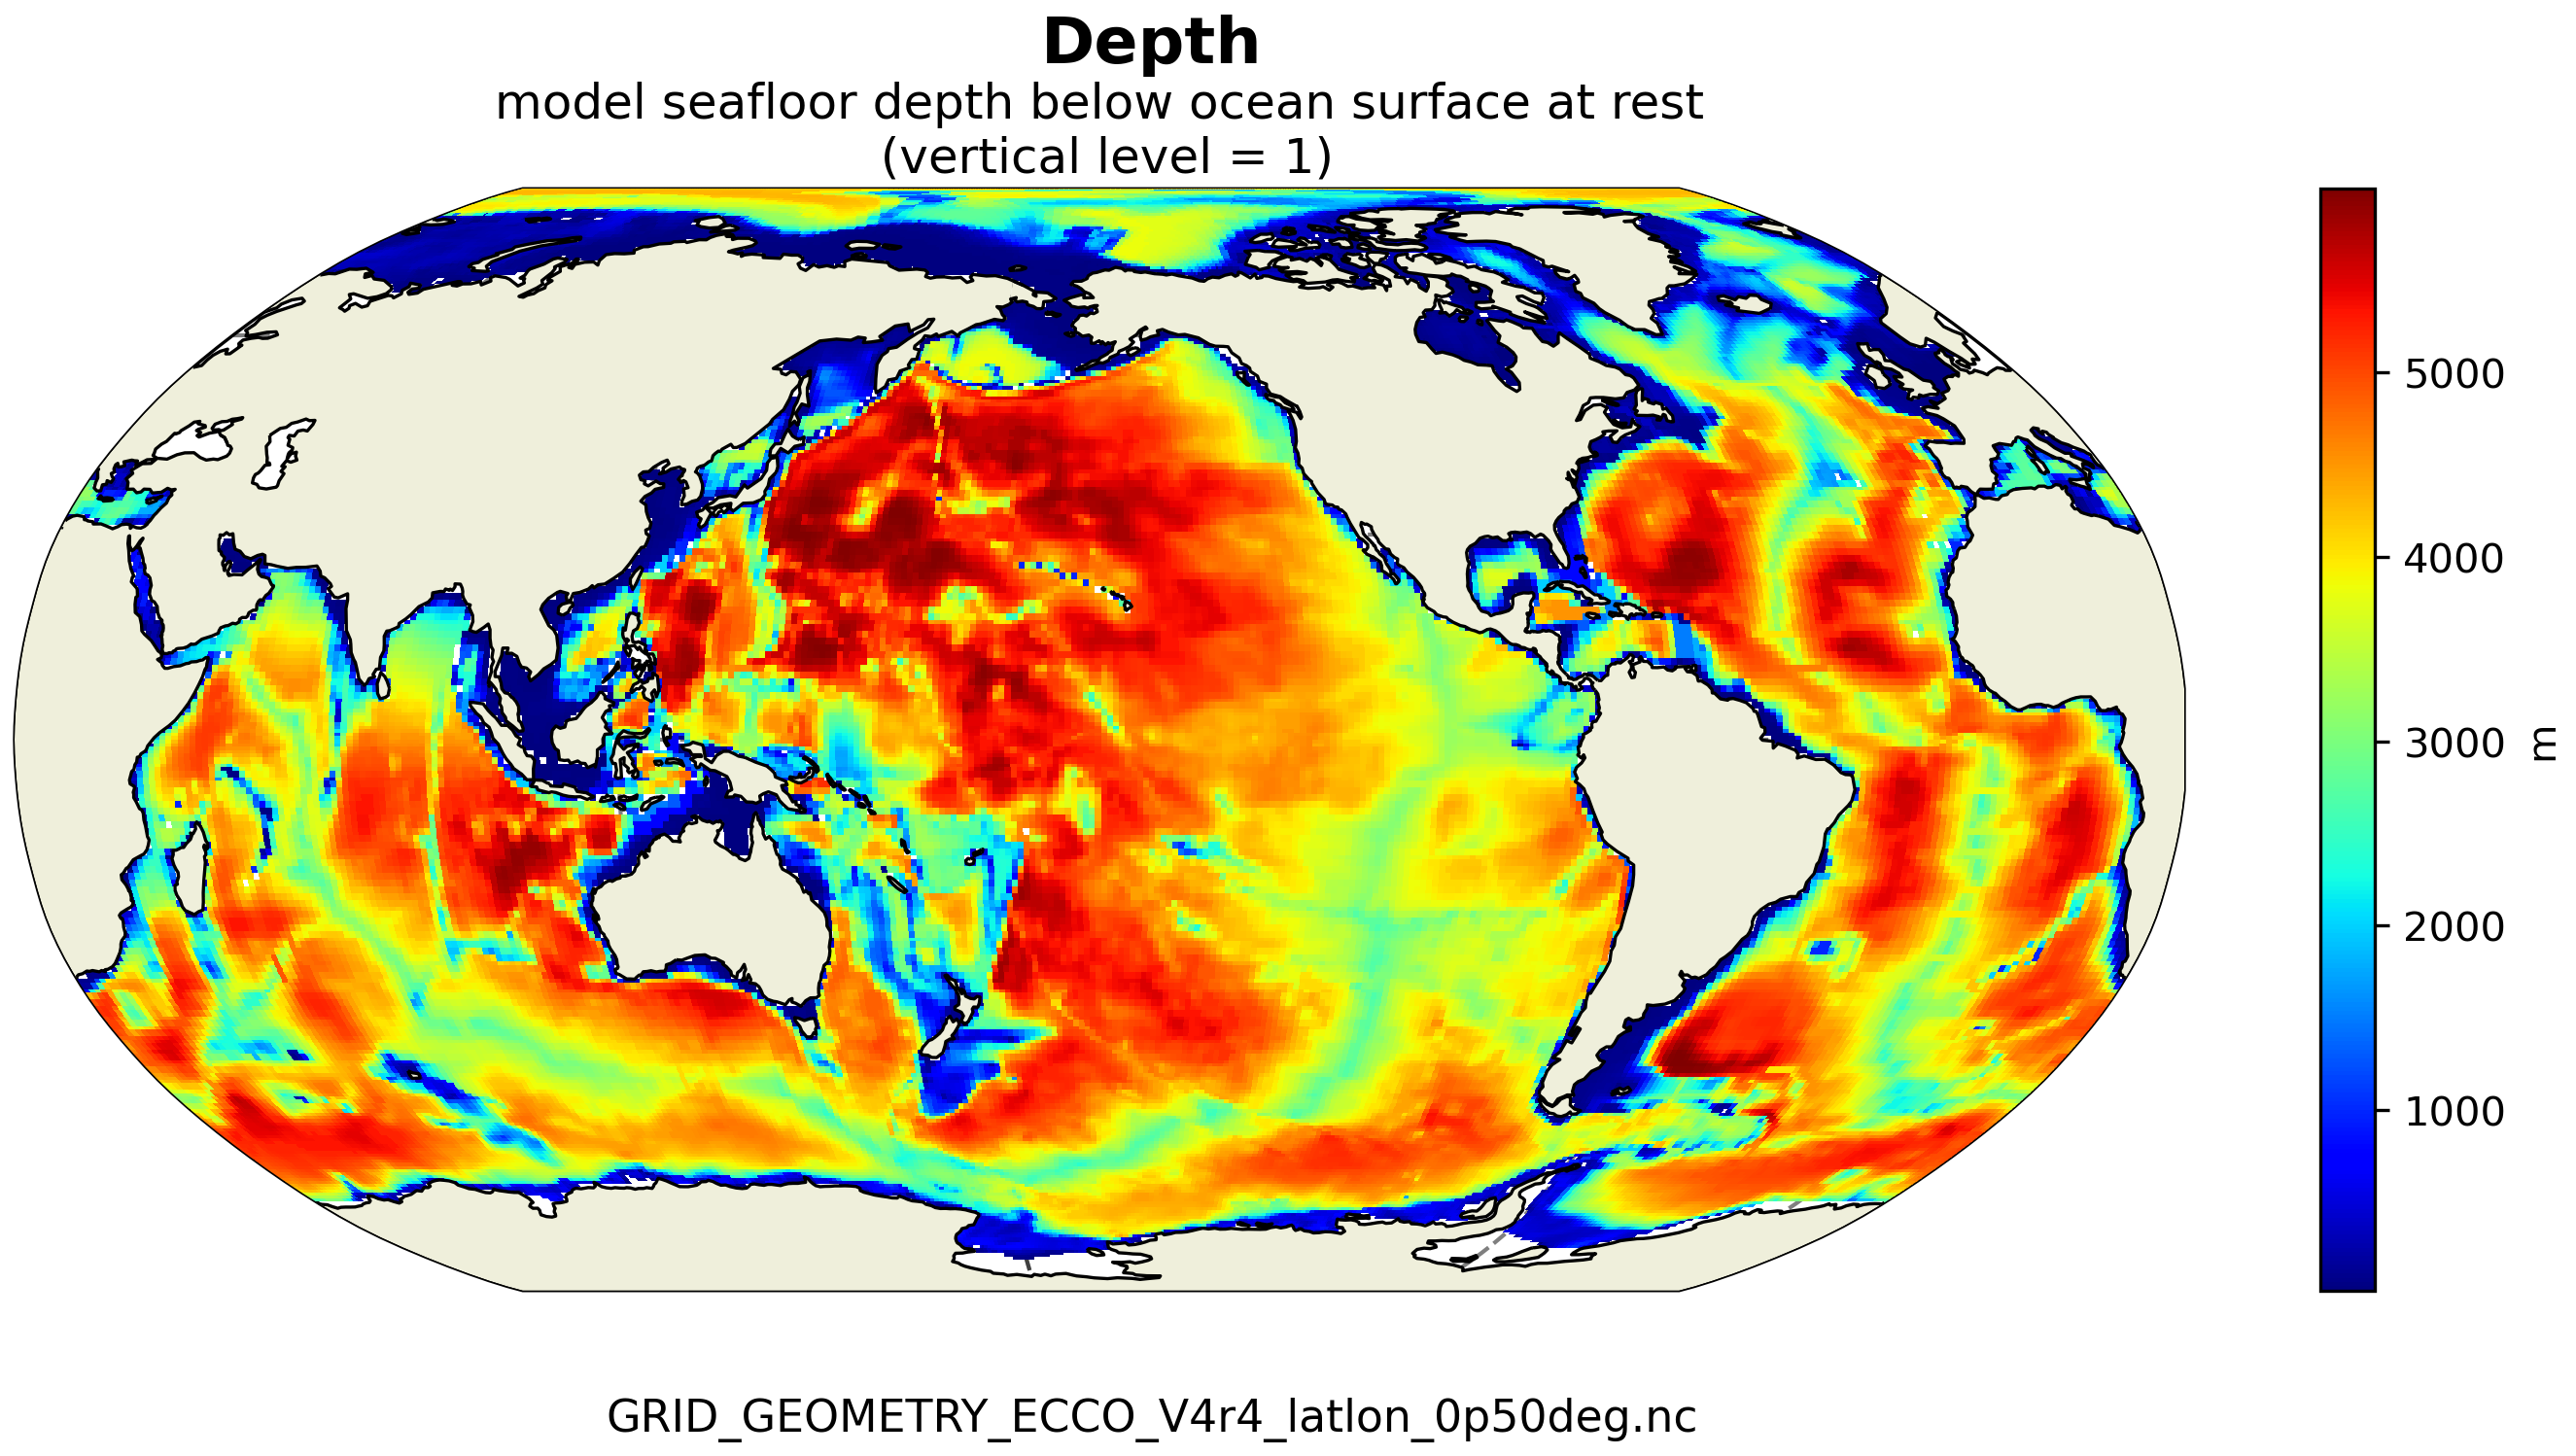
\includegraphics[scale=0.55]{../images/v4r4/plots/latlon_plots_coords/Geometry_Parameters_for_the_0.5_degree_Lat-Lon_Model_Grid_(Version_4_Release_4)/Depth.png}
\caption{Dataset: GRID\_GEOMETRY\_ECCO, Variable: Depth}
\label{tab:table-GRID_GEOMETRY_ECCO_Depth-Plot}
\end{figure}
\newpage
\pagebreak
\subsubsection{Latlon Variable: area}
\begin{longtable}{|m{0.06\textwidth}|m{0.3\textwidth}|m{0.45\textwidth}|m{0.12\textwidth}|}
\caption{Attributes description of the variable 'area' from GRID\_GEOMETRY\_ECCO's  dataset.}
\label{tab:table-GRID_GEOMETRY_ECCO_area} \\ 
\hline \endhead \hline \endfoot
\rowcolor{lightgray} \textbf{Storage Type} & \textbf{Variable Name} & \textbf{Description} & \textbf{Unit} \\ \hline
float64 & area & Area of lat-lon grid cell & m2 \\ \hline
\multicolumn{4}{|c|}{\cellcolor{lightgray}{\textbf{Description of the variable in Common Data language (CDL)}}} \\ \hline
\multicolumn{4}{|c|}{\fontfamily{lmtt}\selectfont{\makecell{\parbox{.95\textwidth}{\vspace*{0.25cm} \footnotesize{float64 area(latitude, longitude)\\
\hspace*{0.5cm}area: \_FillValue = 9.969209968386869e+36\\
\hspace*{0.5cm}area: coverage\_content\_type = modelResult\\
\hspace*{0.5cm}area: long\_name =\hspace*{0.5cm} area of lat-lon grid cell\\
\hspace*{0.5cm}area: standard\_name = cell\hspace*{0.5cm} area\\
\hspace*{0.5cm}area: units = m2\\
}}}}} \\ \hline
\rowcolor{lightgray} \multicolumn{4}{|c|}{\textbf{Comments}} \\ \hline
\multicolumn{4}{|p{1\textwidth}|}{\footnotesize{{N/a}}} \\ \hline
\end{longtable}

\begin{figure}[H]
\centering
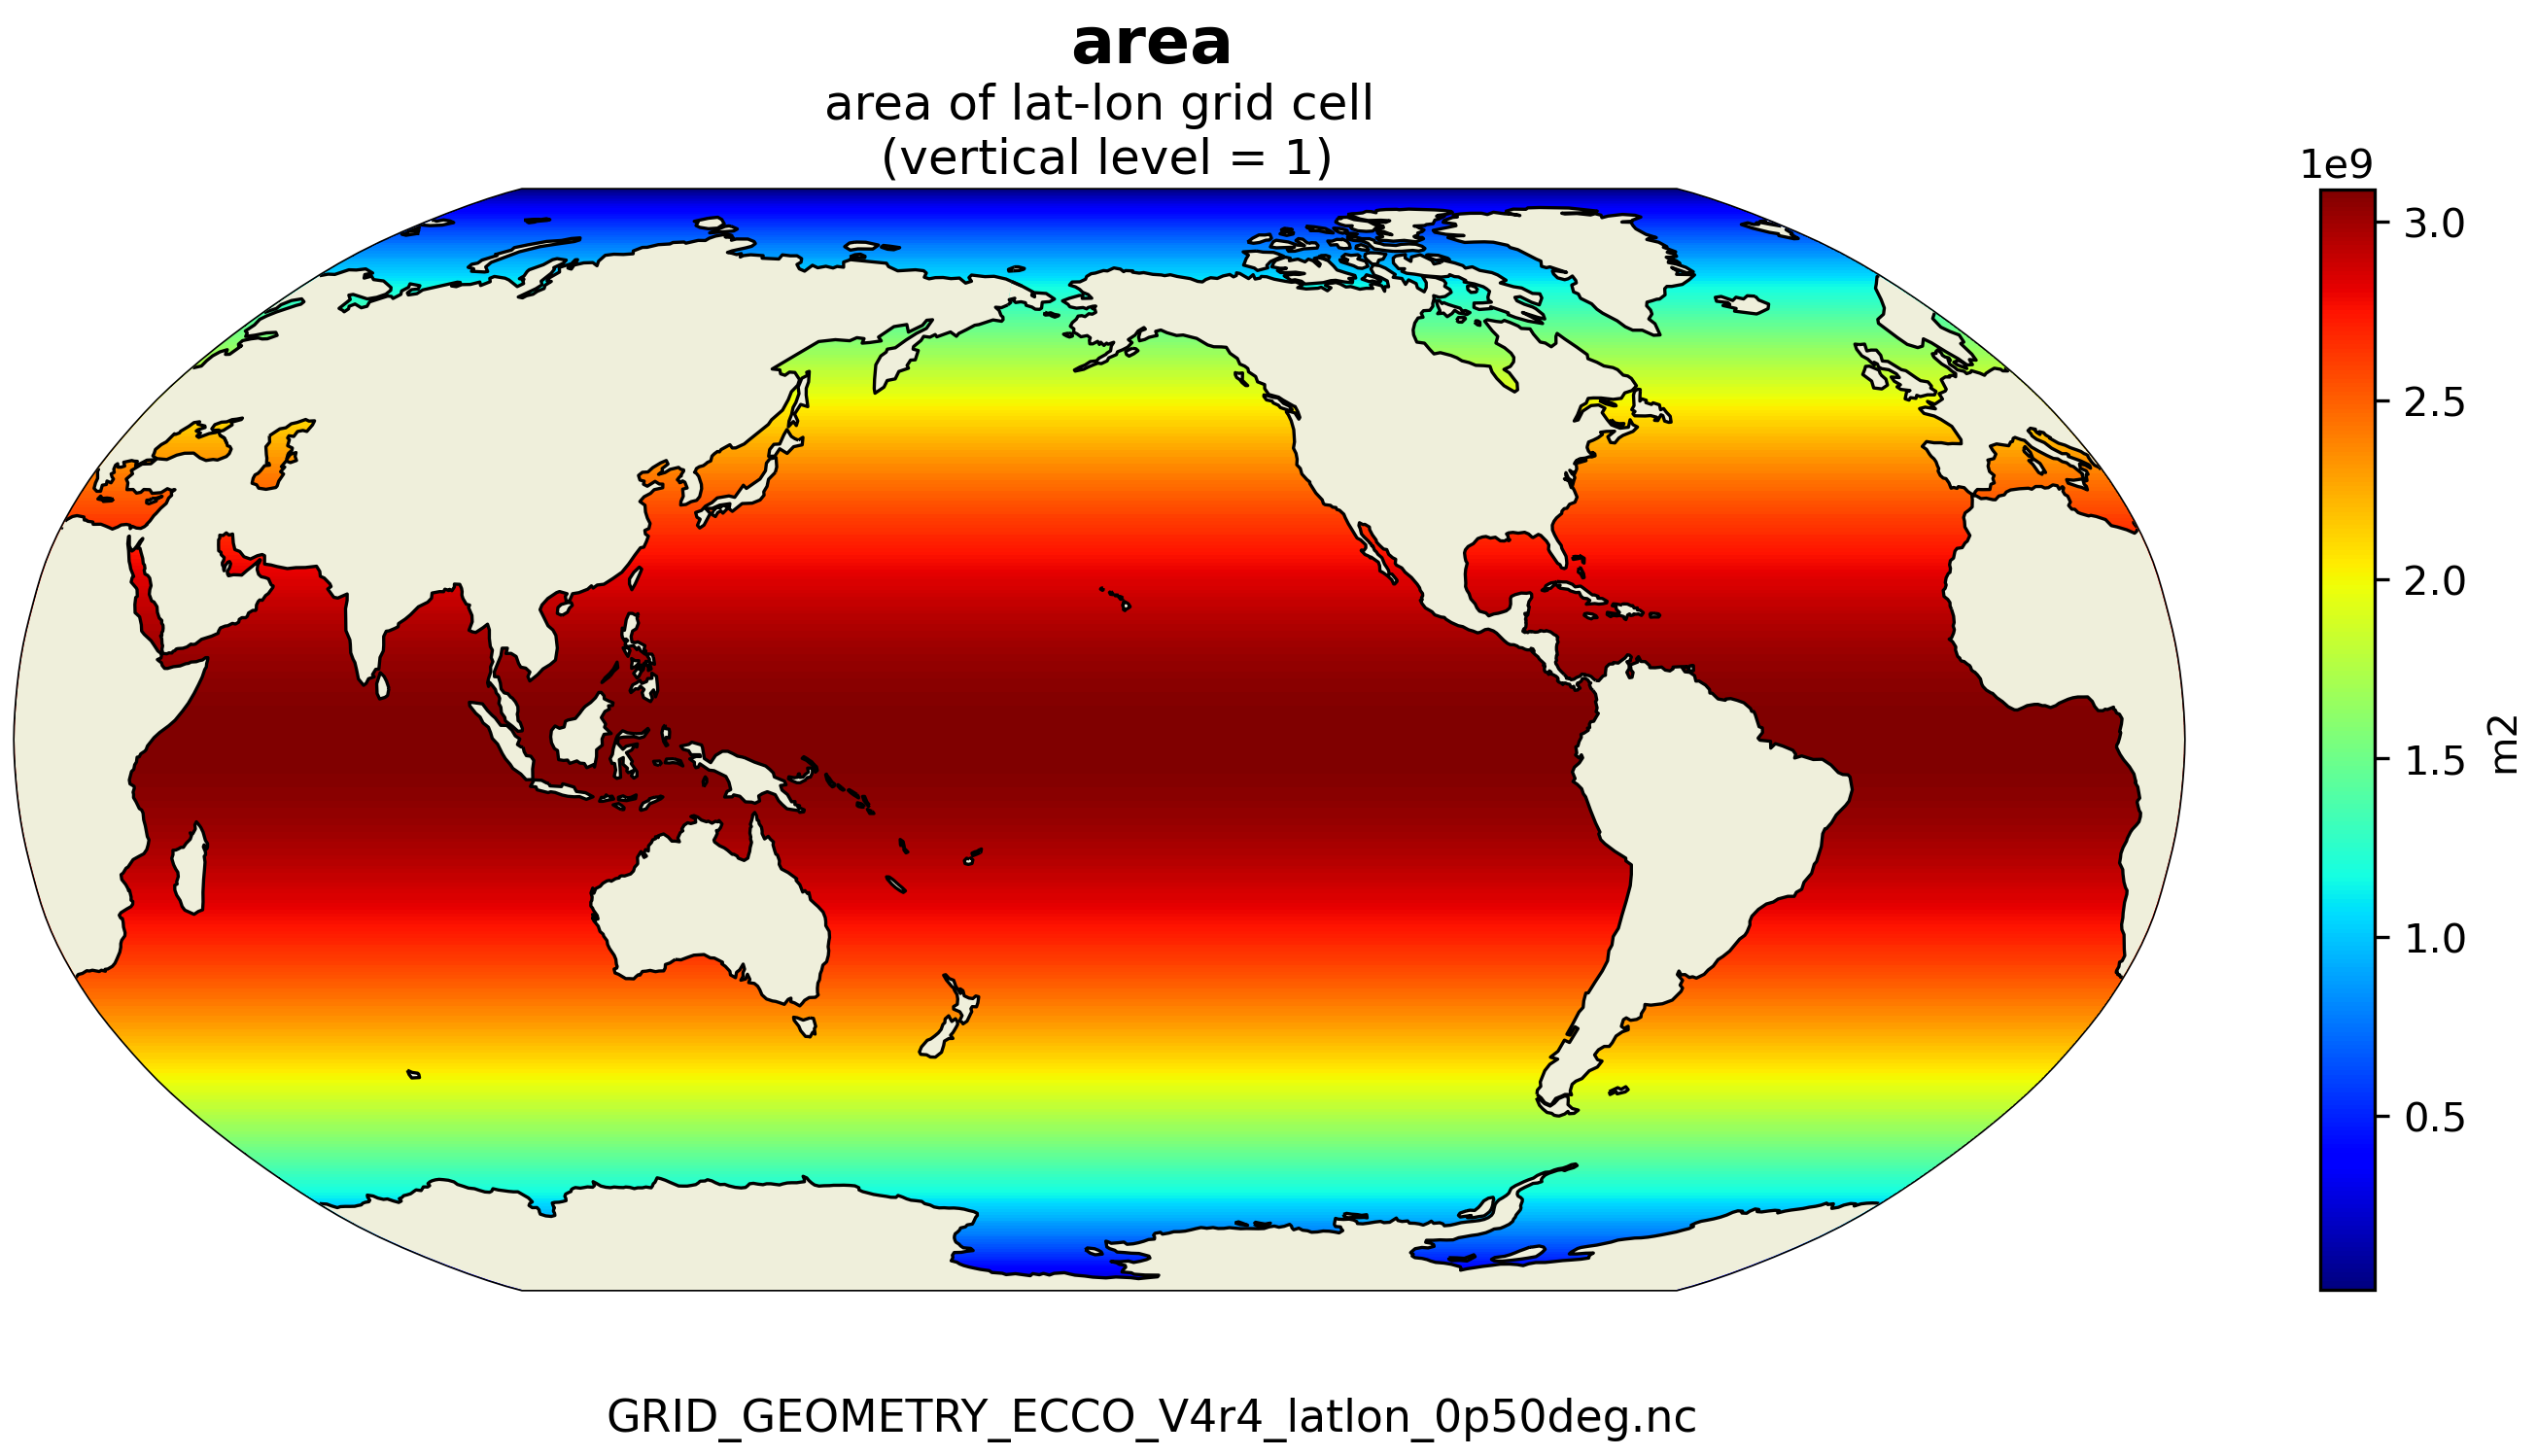
\includegraphics[scale=0.55]{../images/v4r4/plots/latlon_plots_coords/Geometry_Parameters_for_the_0.5_degree_Lat-Lon_Model_Grid_(Version_4_Release_4)/area.png}
\caption{Dataset: GRID\_GEOMETRY\_ECCO, Variable: area}
\label{tab:table-GRID_GEOMETRY_ECCO_area-Plot}
\end{figure}
\newpage
\pagebreak
\subsubsection{Latlon Variable: drF}
\begin{longtable}{|m{0.06\textwidth}|m{0.3\textwidth}|m{0.45\textwidth}|m{0.12\textwidth}|}
\caption{Attributes description of the variable 'drF' from GRID\_GEOMETRY\_ECCO's  dataset.}
\label{tab:table-GRID_GEOMETRY_ECCO_drF} \\ 
\hline \endhead \hline \endfoot
\rowcolor{lightgray} \textbf{Storage Type} & \textbf{Variable Name} & \textbf{Description} & \textbf{Unit} \\ \hline
float32 & drF & Distance between the upper and lower interfaces of the model grid cell & m \\ \hline
\multicolumn{4}{|c|}{\cellcolor{lightgray}{\textbf{Description of the variable in Common Data language (CDL)}}} \\ \hline
\multicolumn{4}{|c|}{\fontfamily{lmtt}\selectfont{\makecell{\parbox{.95\textwidth}{\vspace*{0.25cm} \footnotesize{float32 drF(Z)\\
\hspace*{0.5cm}drF: \_FillValue = 9.96921e+36\\
\hspace*{0.5cm}drF: coverage\_content\_type = modelResult\\
\hspace*{0.5cm}drF: long\_name = distance between the upper and lower interfaces of the model grid cell\\
\hspace*{0.5cm}drF: standard\_name = cell thickness\\
\hspace*{0.5cm}drF: units = m\\
}}}}} \\ \hline
\rowcolor{lightgray} \multicolumn{4}{|c|}{\textbf{Comments}} \\ \hline
\multicolumn{4}{|p{1\textwidth}|}{\footnotesize{{Nominal grid cell thickness.}}} \\ \hline
\end{longtable}

\begin{figure}[H]
\centering
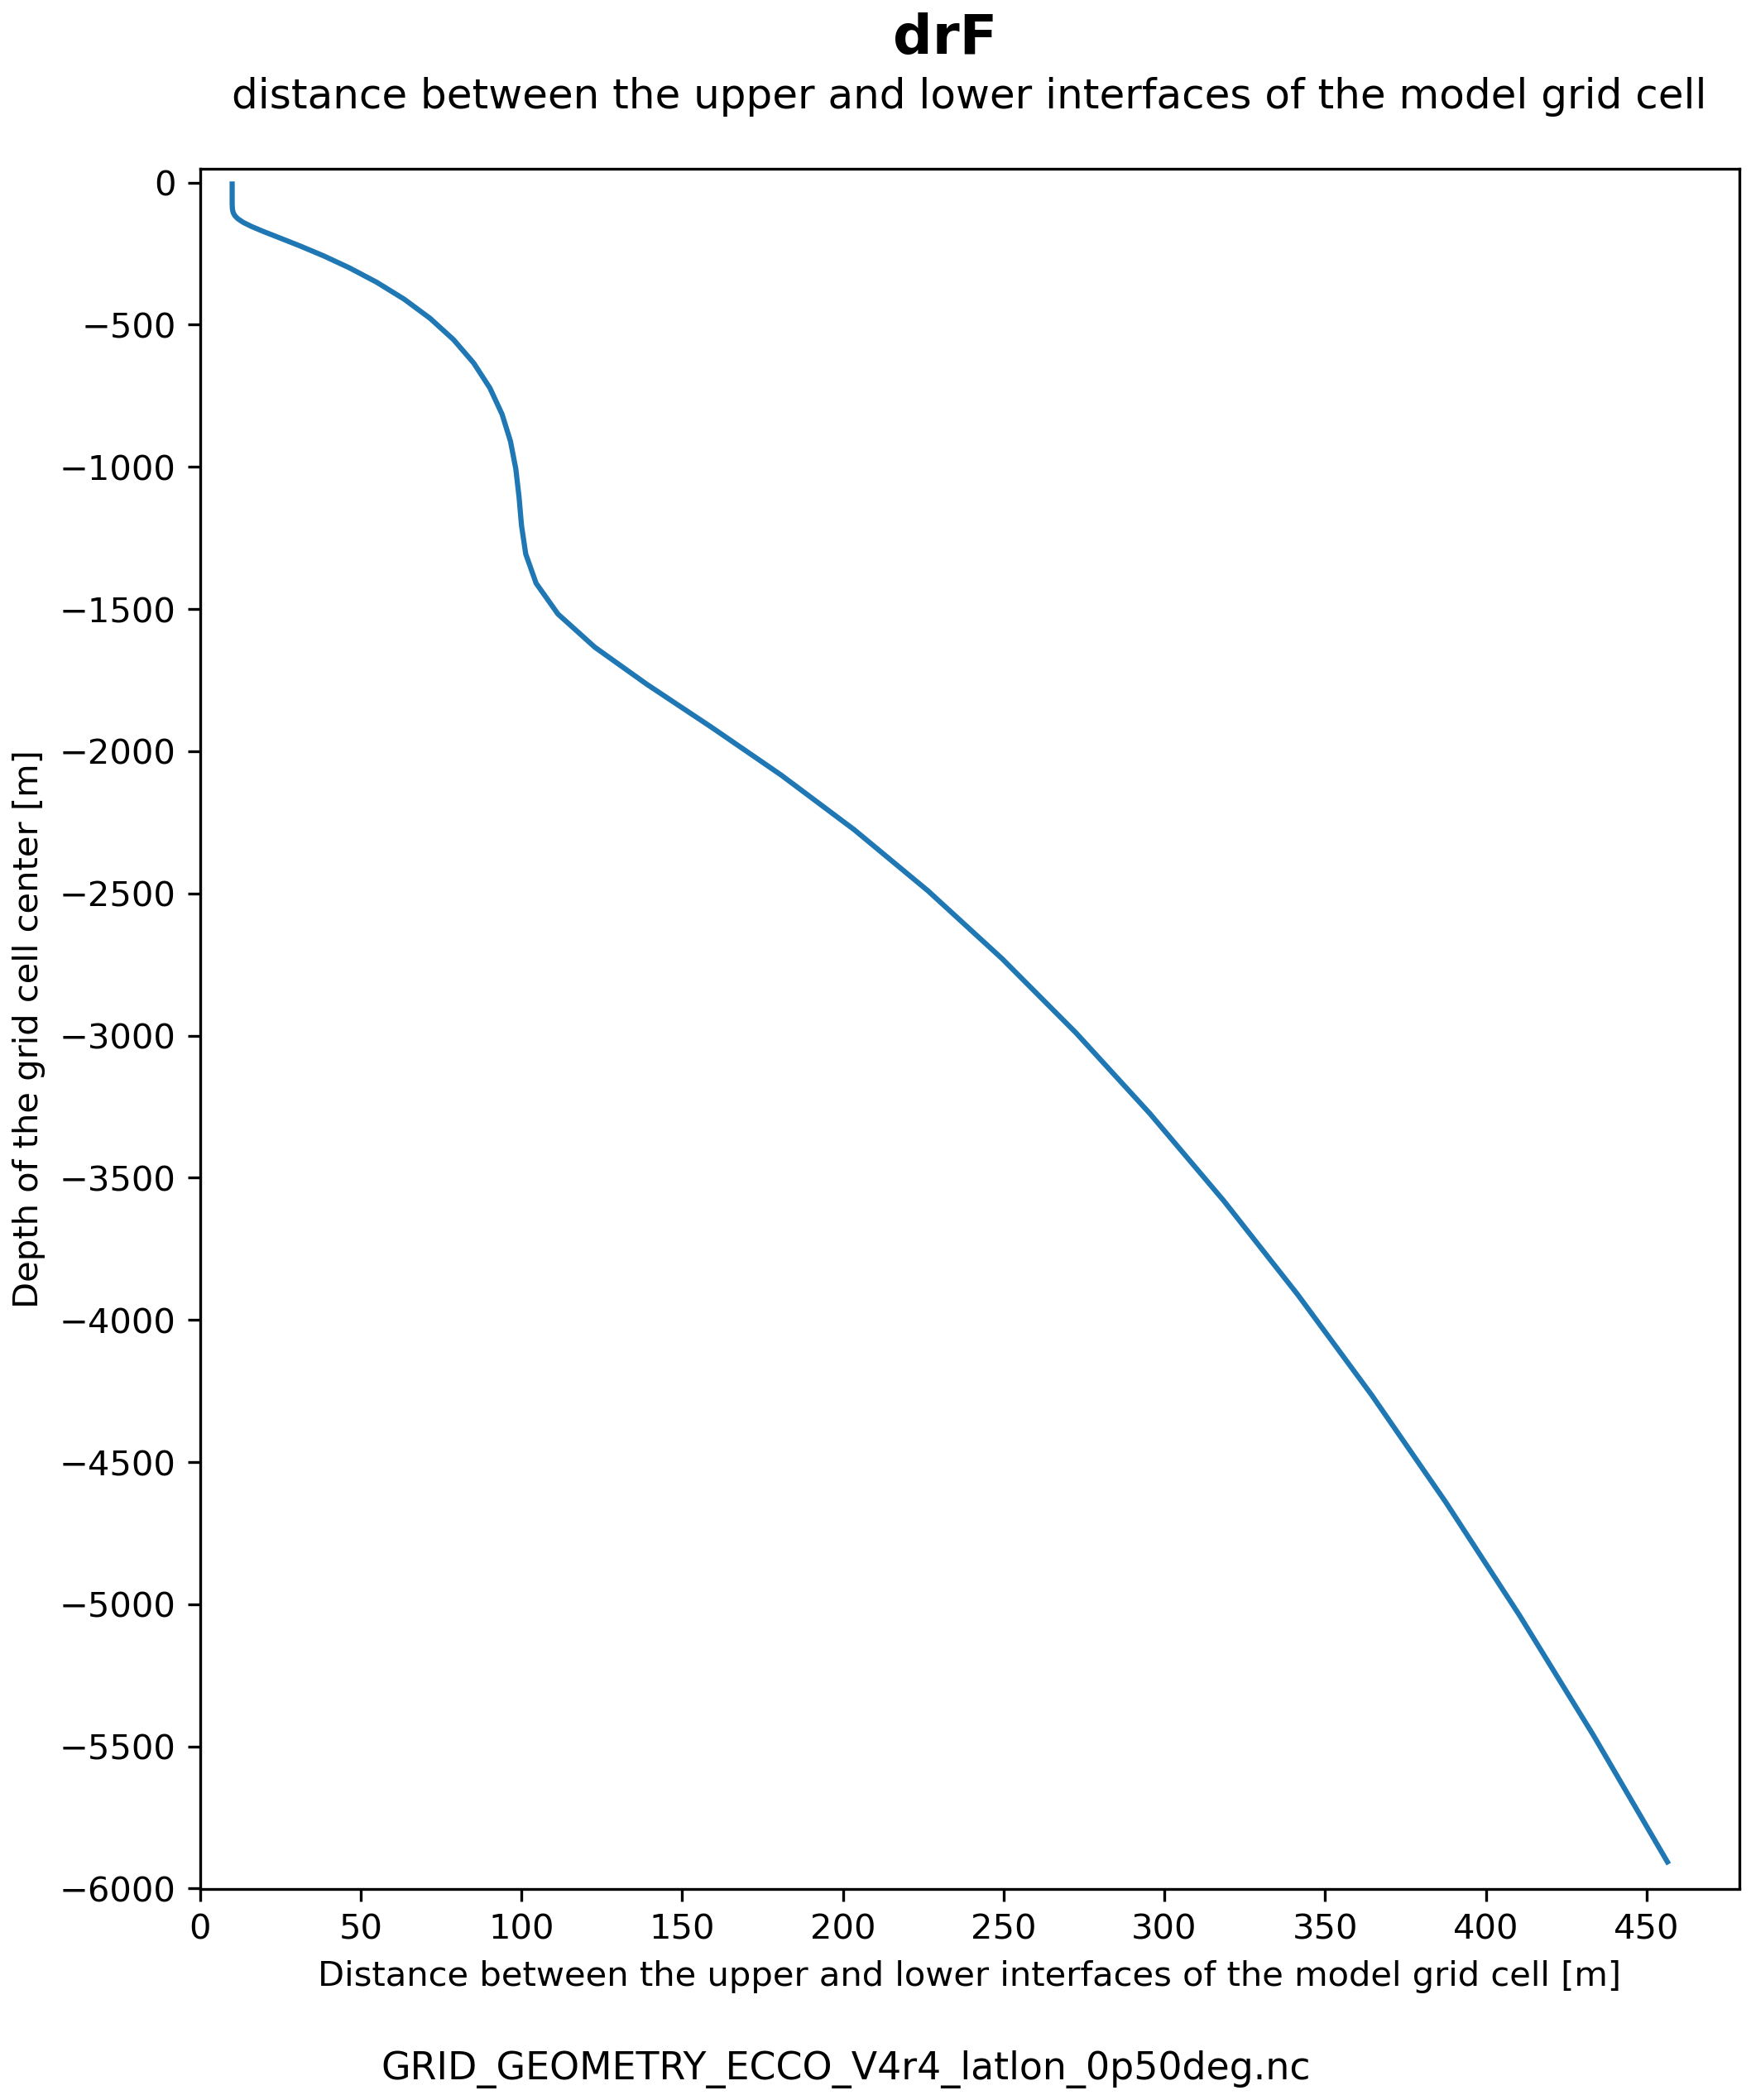
\includegraphics[scale=0.55]{../images/v4r4/plots/latlon_plots_coords/Geometry_Parameters_for_the_0.5_degree_Lat-Lon_Model_Grid_(Version_4_Release_4)/drF.png}
\caption{Dataset: GRID\_GEOMETRY\_ECCO, Variable: drF}
\label{tab:table-GRID_GEOMETRY_ECCO_drF-Plot}
\end{figure}
\newpage
\pagebreak
\subsubsection{Latlon Variable: hFacC}
\begin{longtable}{|m{0.06\textwidth}|m{0.3\textwidth}|m{0.45\textwidth}|m{0.12\textwidth}|}
\caption{Attributes description of the variable 'hFacC' from GRID\_GEOMETRY\_ECCO's  dataset.}
\label{tab:table-GRID_GEOMETRY_ECCO_hFacC} \\ 
\hline \endhead \hline \endfoot
\rowcolor{lightgray} \textbf{Storage Type} & \textbf{Variable Name} & \textbf{Description} & \textbf{Unit} \\ \hline
float64 & hFacC & Vertical open fraction of grid cell & 1 \\ \hline
\multicolumn{4}{|c|}{\cellcolor{lightgray}{\textbf{Description of the variable in Common Data language (CDL)}}} \\ \hline
\multicolumn{4}{|c|}{\fontfamily{lmtt}\selectfont{\makecell{\parbox{.95\textwidth}{\vspace*{0.25cm} \footnotesize{float64 hFacC(Z, latitude, longitude)\\
\hspace*{0.5cm}hFacC: \_FillValue = 9.969209968386869e+36\\
\hspace*{0.5cm}hFacC: coverage\_content\_type = modelResult\\
\hspace*{0.5cm}hFacC: long\_name = vertical open fraction of grid cell\\
\hspace*{0.5cm}hFacC: units = 1\\
}}}}} \\ \hline
\rowcolor{lightgray} \multicolumn{4}{|c|}{\textbf{Comments}} \\ \hline
\multicolumn{4}{|p{1\textwidth}|}{\footnotesize{{Grid cells may be fractionally closed in the vertical. the open vertical fraction is hfacc. the model allows for partially-filled cells to represent topographic variations more smoothly (hfacc < 1). completely closed (dry) tracer grid cells have hfacc = 0. note: the lat-lon gridded hfacc is spatially-averaged from the hfacc field on the lat-lon-cap (llc90) model native grid. the total ocean volume of the ecco v4r4 lat-lon gridded fields is within 0.05\% of the total ocean volume of the native grid fields.}}} \\ \hline
\end{longtable}

\begin{figure}[H]
\centering
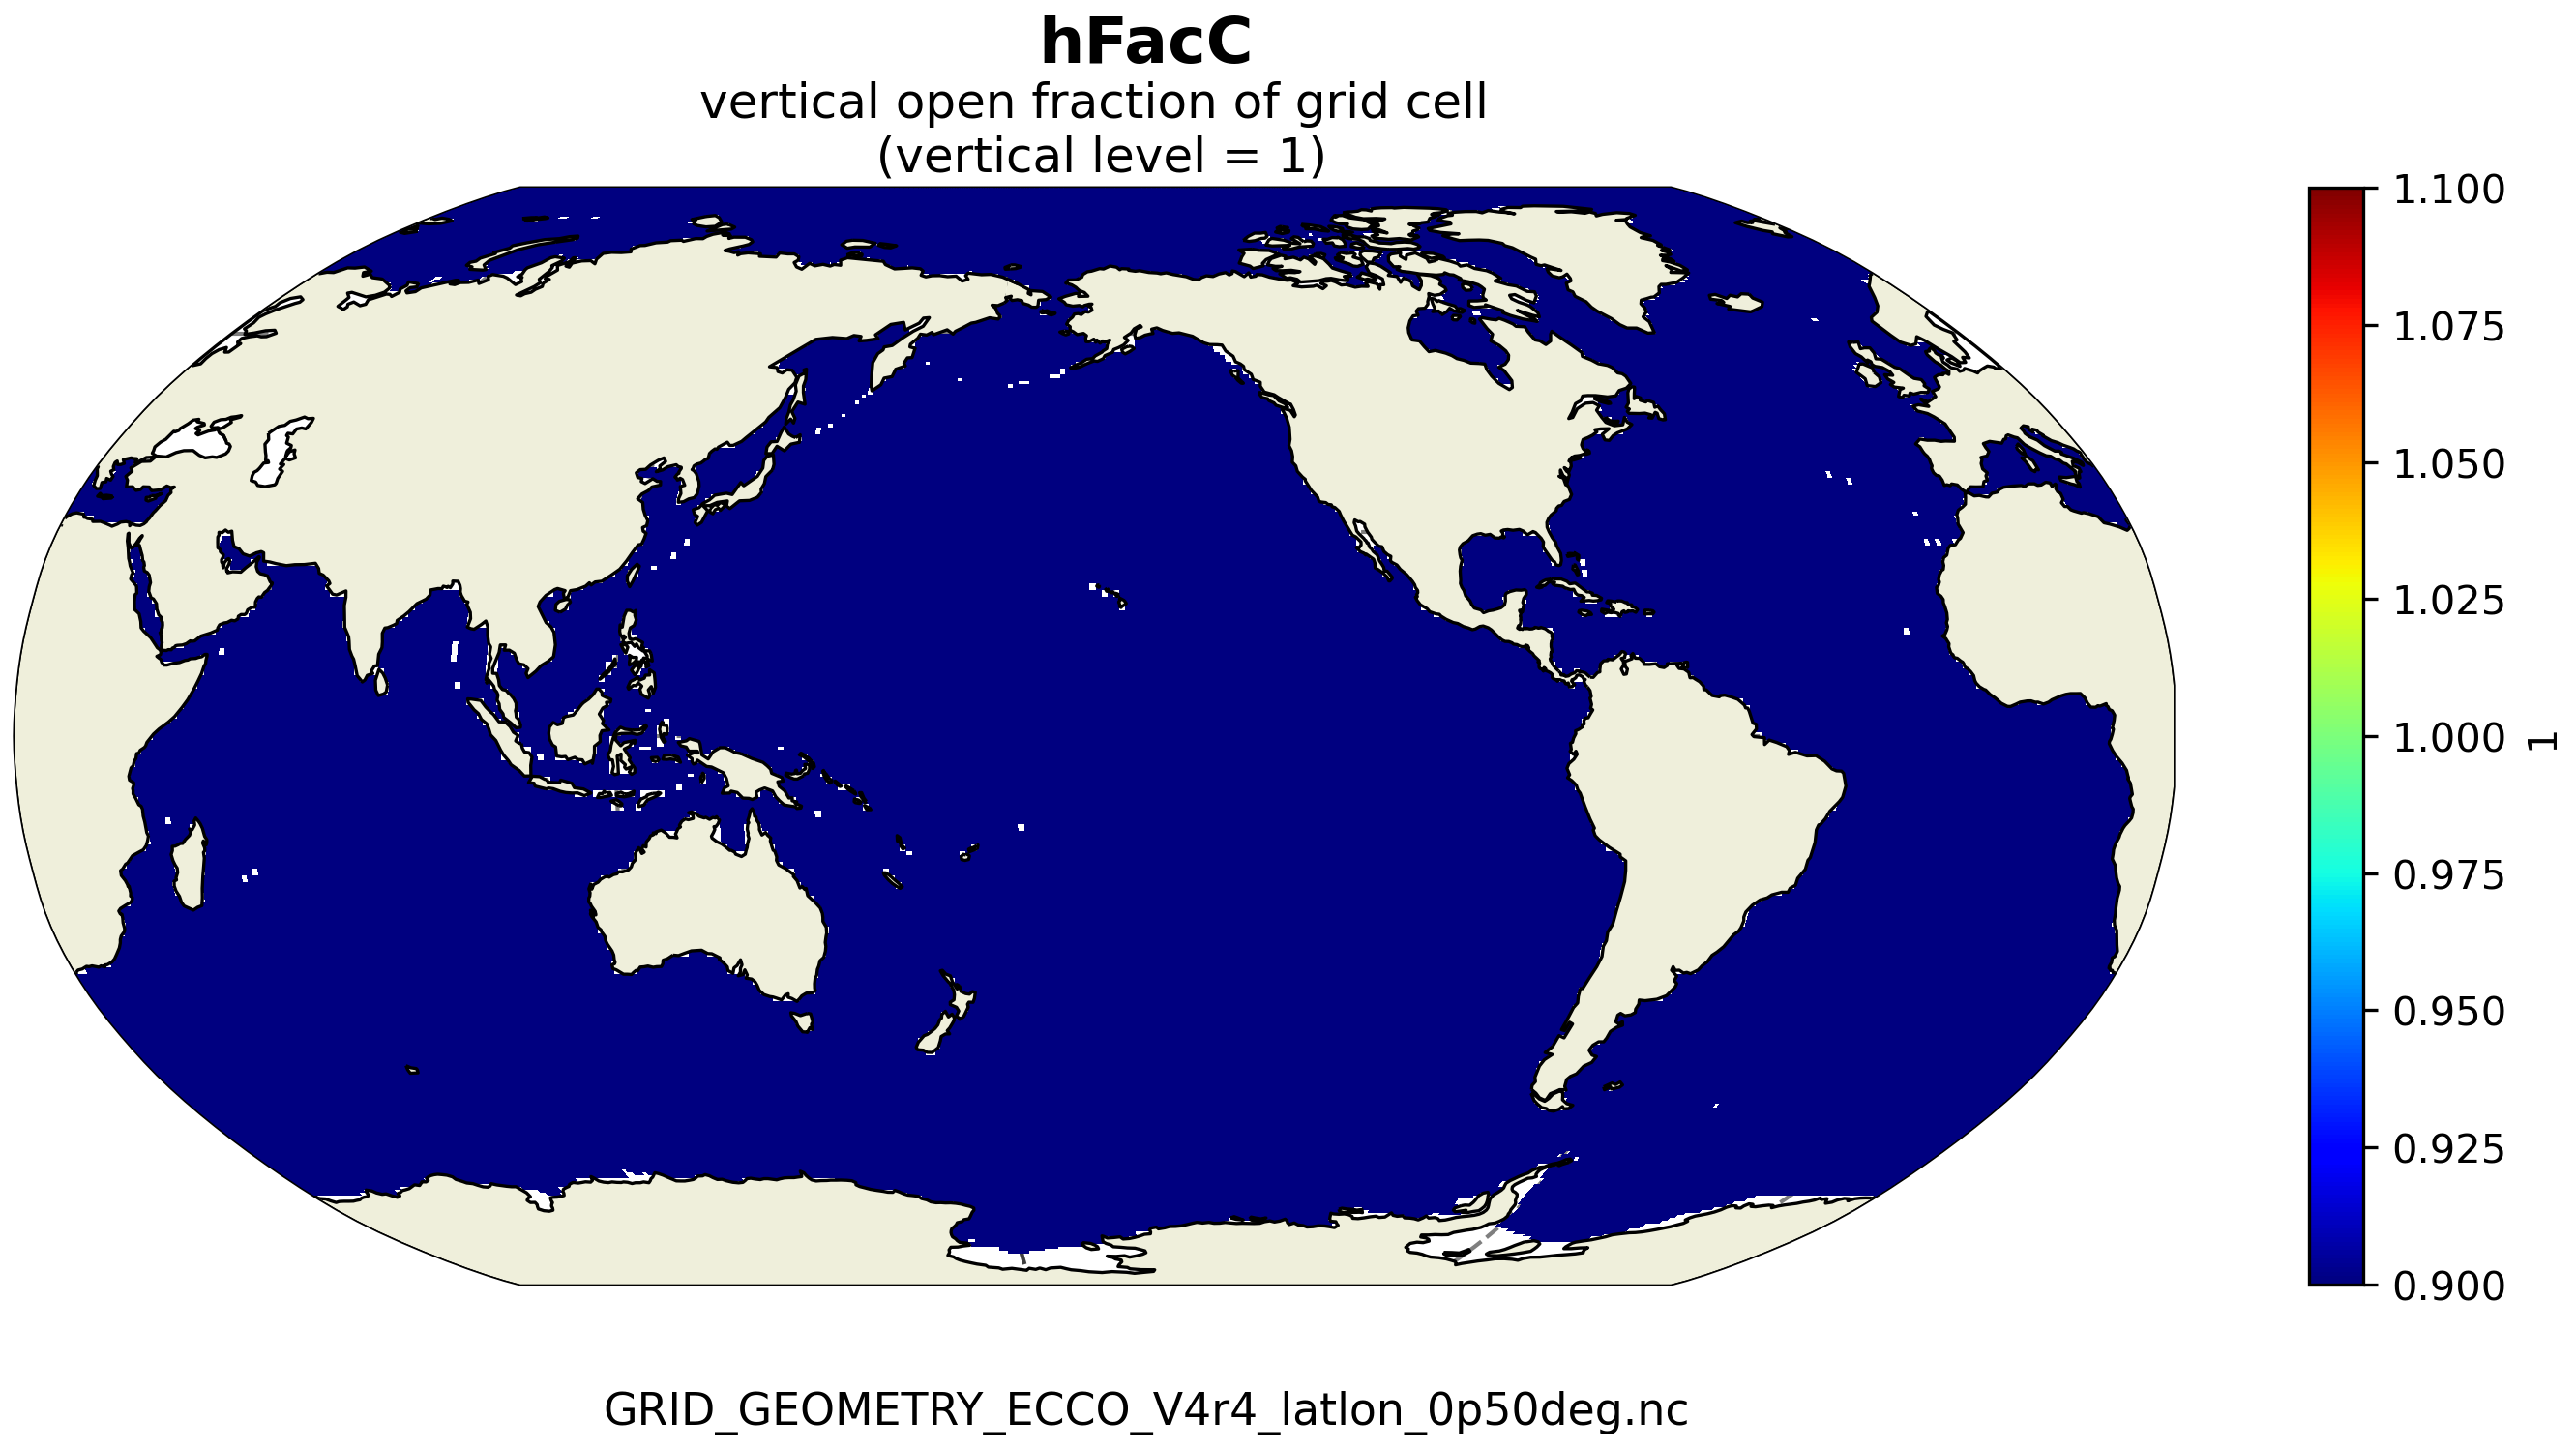
\includegraphics[scale=0.55]{../images/v4r4/plots/latlon_plots_coords/Geometry_Parameters_for_the_0.5_degree_Lat-Lon_Model_Grid_(Version_4_Release_4)/hFacC.png}
\caption{Dataset: GRID\_GEOMETRY\_ECCO, Variable: hFacC}
\label{tab:table-GRID_GEOMETRY_ECCO_hFacC-Plot}
\end{figure}
\newpage
\pagebreak
\subsubsection{Latlon Variable: maskC}
\begin{longtable}{|m{0.06\textwidth}|m{0.3\textwidth}|m{0.45\textwidth}|m{0.12\textwidth}|}
\caption{Attributes description of the variable 'maskC' from GRID\_GEOMETRY\_ECCO's  dataset.}
\label{tab:table-GRID_GEOMETRY_ECCO_maskC} \\ 
\hline \endhead \hline \endfoot
\rowcolor{lightgray} \textbf{Storage Type} & \textbf{Variable Name} & \textbf{Description} & \textbf{Unit} \\ \hline
bool & maskC & Wet/dry boolean mask for grid cell & N/A \\ \hline
\multicolumn{4}{|c|}{\cellcolor{lightgray}{\textbf{Description of the variable in Common Data language (CDL)}}} \\ \hline
\multicolumn{4}{|c|}{\fontfamily{lmtt}\selectfont{\makecell{\parbox{.95\textwidth}{\vspace*{0.25cm} \footnotesize{bool maskC(Z, latitude, longitude)\\
\hspace*{0.5cm}maskC: \_FillValue = 1\\
\hspace*{0.5cm}maskC: coverage\_content\_type = modelResult\\
\hspace*{0.5cm}maskC: long\_name = wet/dry boolean mask for grid cell\\
}}}}} \\ \hline
\rowcolor{lightgray} \multicolumn{4}{|c|}{\textbf{Comments}} \\ \hline
\multicolumn{4}{|p{1\textwidth}|}{\footnotesize{{True for grid cells with nonzero open vertical fraction (hfacc > 0), otherwise false.}}} \\ \hline
\end{longtable}

\begin{figure}[H]
\centering
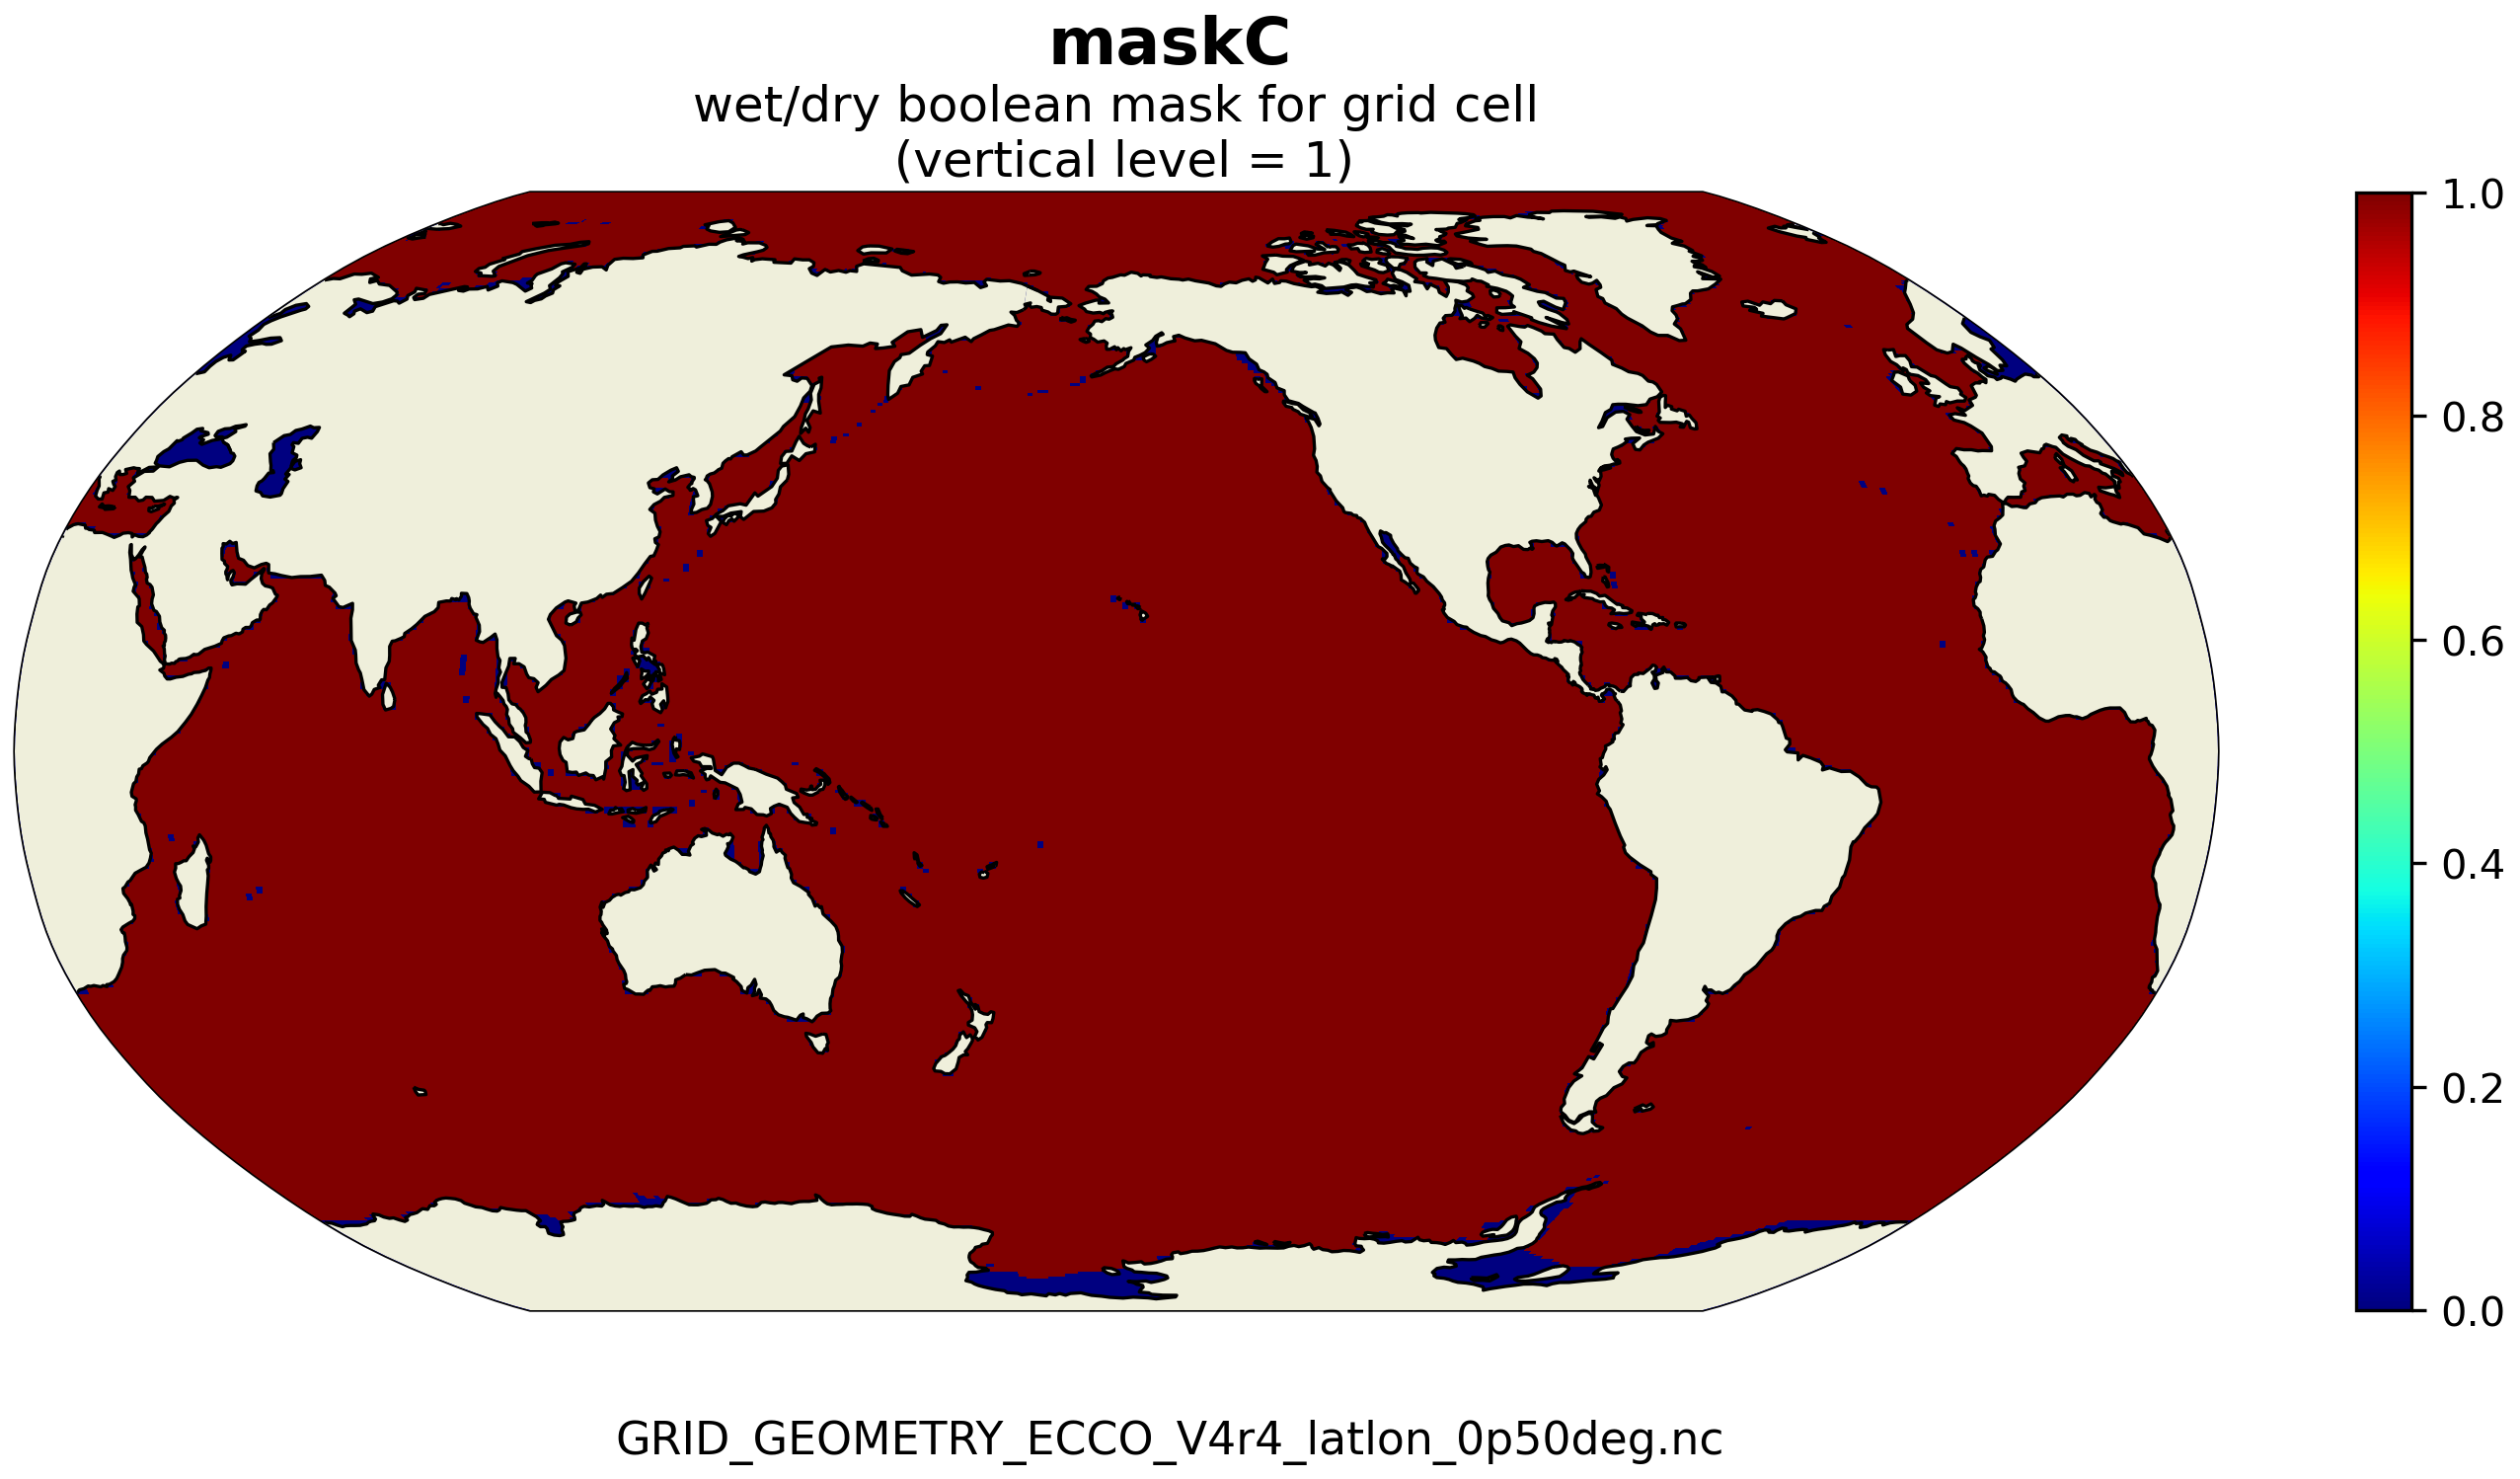
\includegraphics[scale=0.55]{../images/v4r4/plots/latlon_plots_coords/Geometry_Parameters_for_the_0.5_degree_Lat-Lon_Model_Grid_(Version_4_Release_4)/maskC.png}
\caption{Dataset: GRID\_GEOMETRY\_ECCO, Variable: maskC}
\label{tab:table-GRID_GEOMETRY_ECCO_maskC-Plot}
\end{figure}
\newpage